\section{Optimizers}
\begin{frame}{The Three Pillars of Learning}
    \centering
    \begin{tikzpicture}[
        scale=0.85, transform shape, 
        node distance=1.0cm and 0.3cm,
        box/.style={
            rectangle, rounded corners, draw=none, 
            text width=4.0cm, minimum height=1.8cm, 
            align=center, font=\small
        },
        title/.style={font=\bfseries\large},
    ]
        % --- Column 1: The Model (Dimmed) ---
        \node[title, blue, opacity=0.4] (h_title) at (0,0) {1. The Model ($f_\theta$)};
        \node[box, fill=blue!10, text=gray, opacity=0.5, below=0.2cm of h_title] (h_box) {
            \textbf{Design Choice:}\\
            Neural Networks \\ (Architecture)
        };

        % --- Column 2: Loss Function (Dimmed) ---
        \node[title, red, opacity=0.4] (l_title) at (4.5,0) {2. Loss Function ($J$)};
        \node[box, fill=red!10, text=gray, opacity=0.5, below=0.2cm of l_title] (l_box) {
            \textbf{Design Choice:}\\
            MSE / Cross-Entropy
        };

        % --- Column 3: Optimizer (ACTIVE) ---
        \node[title, green!60!black] (o_title) at (9.0,0) {3. Optimizer};
        \node[box, fill=green!10, below=0.2cm of o_title] (o_box) {
            \textbf{Design Choice:}\\
            SGD, Adam, RMSProp
            \vspace{0.5em}
            
            \textbf{Depends on:}\\
            Stability \& Convergence Speed
        };
    \end{tikzpicture}

    \vspace{1em}
    \begin{block}{}
        We defined the Models (1) and the Losses (2). \\
        Now, Let's discuss optimizers.
    \end{block}
\end{frame}


% --- Gradient Descent: Intuition ---
\begin{frame}{Gradient Descent: The Core Idea}
\textbf{Goal:} Find parameters $\theta$ that minimize the loss $J(\theta)$.

\textbf{Intuition:} Follow the negative gradient (steepest descent direction).

\vspace{0.5em}
\centering
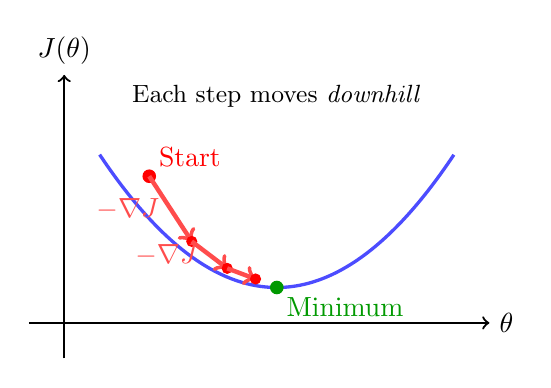
\begin{tikzpicture}[scale=0.9]
    % Draw loss surface
    \draw[->, thick] (-0.5,0) -- (6,0) node[right] {$\theta$};
    \draw[->, thick] (0,-0.5) -- (0,3.5) node[above] {$J(\theta)$};
    
    % Loss curve (parabola-like)
    \draw[blue!70, very thick, domain=0.5:5.5, samples=100] 
        plot (\x, {0.3*(\x-3)^2 + 0.5});
    
    % Starting point
    \filldraw[red] (1.2, 2.07) circle (2.5pt) node[above right] {Start};
    
    % Gradient arrows and steps
    \draw[->, red!70, ultra thick] (1.2, 2.07) -- (1.8, 1.15) node[midway, left] {$-\nabla J$};
    \filldraw[red] (1.8, 1.15) circle (2pt);
    
    \draw[->, red!70, ultra thick] (1.8, 1.15) -- (2.3, 0.77) node[midway, left] {$-\nabla J$};
    \filldraw[red] (2.3, 0.77) circle (2pt);
    
    \draw[->, red!70, ultra thick] (2.3, 0.77) -- (2.7, 0.62);
    \filldraw[red] (2.7, 0.62) circle (2pt);
    
    % Minimum
    \filldraw[green!60!black] (3, 0.5) circle (2.5pt) node[below right] {Minimum};
    
    \node[font=\small] at (3, 3.2) {Each step moves \textit{downhill}};
\end{tikzpicture}

\vspace{0.5em}
The gradient $\nabla_\theta J(\theta)$ tells us which direction increases the loss most.\\
We go the \textbf{opposite direction} to decrease it.
\end{frame}

% --- Gradient Descent: Math ---
\begin{frame}{Gradient Descent: Update Rule}
\textbf{Basic update equation:}
\[
\theta_{\text{new}} = \theta_{\text{old}} - \alpha \nabla_\theta J(\theta)
\]

\begin{itemize}
\item $\alpha$ is the \textbf{learning rate} (step size)
\item $\nabla_\theta J(\theta)$ is the gradient of loss w.r.t. parameters
\item Repeat until convergence (or for fixed number of steps)
\end{itemize}

\pause
\vspace{0.5em}
\textbf{Three variants based on how much data we use:}
\begin{enumerate}
\item \textbf{Batch Gradient Descent:} Use entire dataset
\item \textbf{Stochastic Gradient Descent (SGD):} Use one sample
\item \textbf{Mini-Batch Gradient Descent:} Use small batch of samples
\end{enumerate}
\end{frame}
% --- Batch vs Mini-Batch vs Stochastic: Intuition ---
\begin{frame}{Batch GD vs Mini-Batch GD vs Stochastic GD}
    \textbf{How much data do we use per update (one step)?}
    
    \vspace{0.8em}
    \centering
    \begin{tikzpicture}[
        font=\footnotesize,
        node distance=1.2cm and 0.3cm, % Vertical and Horizontal spacing
        box/.style={draw, rounded corners, thick, align=center, minimum height=1.2cm, minimum width=3.5cm},
        dataset/.style={box, fill=gray!10, minimum width=10cm, minimum height=0.8cm},
        arr/.style={->, thick, >=latex}, % Added arrow tip style
        dot/.style={circle, draw, fill=white, inner sep=1.5pt}
    ]
        % 1. Top Dataset
        \node[dataset] (D) {Full Training Dataset};
        
        % 2. The Methods (Positioning: Center first, then Left/Right)
        \node[box, fill=green!10, below=of D] (MB) {\textbf{Mini-Batch GD}\\[-0.5ex]\scriptsize (uses a batch)};
        \node[box, fill=blue!10, left=of MB] (BGD) {\textbf{Batch GD}\\[-0.5ex]\scriptsize (uses all data)};
        \node[box, fill=red!10, right=of MB] (SGD) {\textbf{Stochastic GD}\\[-0.5ex]\scriptsize (uses 1 sample)};
        
        % 3. Arrows
        \draw[arr] (D.south) -- (MB.north);
        \draw[arr] (D.south) -- (BGD.north);
        \draw[arr] (D.south) -- (SGD.north);
        
        % 4. Dots (Visuals - Centered relative to box center)
        % Batch: Row of dots
        \foreach \x in {-1.2, -0.8, -0.4, 0, 0.4, 0.8, 1.2}
            \node[dot] at ($(BGD.center) + (\x, -0.4)$) {};
            
        % Mini-Batch: Few dots
        \foreach \x in {-0.4, 0, 0.4}
            \node[dot] at ($(MB.center) + (\x, -0.4)$) {};
            
        % Stochastic: One dot
        \node[dot] at ($(SGD.center) + (0, -0.4)$) {};
    
    \end{tikzpicture}
    
    \vspace{1em}
    
    % Text Columns
    \begin{columns}[t]
        \begin{column}{0.33\textwidth}
            \textbf{Batch GD}
            \footnotesize
            \begin{itemize}
                \item Stable updates
                \item Expensive per step
                \item Needs lots of RAM
            \end{itemize}
        \end{column}
        
        \begin{column}{0.33\textwidth}
            \textbf{Mini-Batch (Default)}
            \footnotesize
            \begin{itemize}
                \item Best of both worlds
                \item Stable \& Fast
                \item GPU Efficient
            \end{itemize}
        \end{column}
        
        \begin{column}{0.33\textwidth}
            \textbf{Stochastic GD}
            \footnotesize
            \begin{itemize}
                \item Very noisy updates
                \item Can escape local minima
                \item Slow (can't parallelize)
            \end{itemize}
        \end{column}
    \end{columns}
    
    \vspace{0.5em}
    \centering
    \small \textit{In practice: we almost always use Mini-Batch (whenever GD mentioned next, it refers to the mini-batch variant).}
\end{frame}

% --- Batch vs Mini-Batch vs Stochastic: Convergence Plot ---
% --- Slide: Convergence Paths (Separated Directions) ---
\begin{frame}{Convergence Behavior}
    \textbf{How do they navigate the Loss Surface?}
    
    \vspace{0.5em}
    \centering
    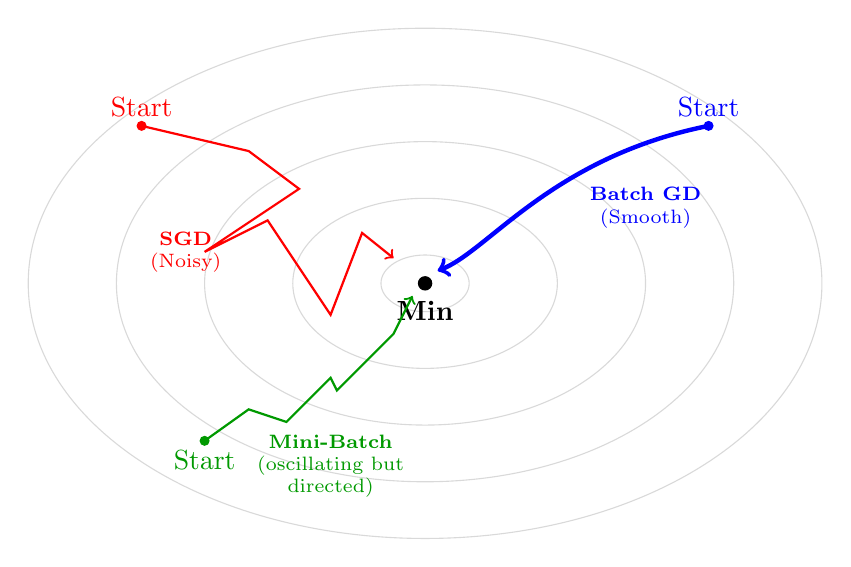
\begin{tikzpicture}[scale=0.8]
        % --- 1. Draw Contours (The Loss Landscape) ---
        \foreach \r in {0.5, 1.5, 2.5, 3.5, 4.5} {
            \draw[gray!30, thin] (0,0) ellipse ({1.4*\r} and {0.9*\r});
        }
        % Minimum Point
        \filldraw[black] (0,0) circle (3pt) node[below=3pt, font=\bfseries] {Min};

        % --- 2. Batch GD (Blue) - Smooth & Direct ---
        % Starts Top-Right
        \coordinate (batch_start) at (4.5, 2.5);
        \filldraw[blue] (batch_start) circle (2pt) node[above] {Start};
        \draw[blue, ultra thick, ->] (batch_start) 
            .. controls (2.0, 2.0) and (1.0, 0.5) .. (0.2, 0.2);
        \node[blue, font=\scriptsize, align=center] at (3.5, 1.2) {\textbf{Batch GD}\\(Smooth)};

        % --- 3. SGD (Red) - Chaotic ZigZag ---
        % Starts Top-Left
        \coordinate (sgd_start) at (-4.5, 2.5);
        \filldraw[red] (sgd_start) circle (2pt) node[above] {Start};
        \draw[red, thick, ->] plot coordinates {
            (-4.5, 2.5) (-2.8, 2.1) (-2.0, 1.5) (-3.5, 0.5) 
            (-2.5, 1.0) (-1.5, -0.5) (-1.0, 0.8) (-0.5, 0.4) 
        };
        \node[red, font=\scriptsize, align=center] at (-3.8, 0.5) {\textbf{SGD}\\(Noisy)};

        % --- 4. Mini-Batch (Green) - Slight Wiggle ---
        % Starts Bottom-Left
        \coordinate (mb_start) at (-3.5, -2.5);
        \filldraw[green!60!black] (mb_start) circle (2pt) node[below] {Start};
        \draw[green!60!black, thick, ->] plot coordinates {
            (-3.5, -2.5) (-2.8, -2.0) (-2.2, -2.2) (-1.5, -1.5) 
            (-1.4, -1.7) (-0.5, -0.8) (-0.2, -0.2)
        };
        \node[green!60!black, font=\scriptsize, align=center] at (-1.5, -2.9) {\textbf{Mini-Batch}\\(oscillating but\\directed)};

    \end{tikzpicture}

\end{frame}
% --- Momentum: Intuition (Dampened Oscillation) --- 
\begin{frame}{Momentum: Adding Inertia} 
    \textbf{The Ravine Problem:} 
    Gradient Descent makes slow progress because it "bounces" off the steep walls. 
     
    \vspace{0.5em} 
    \centering 
    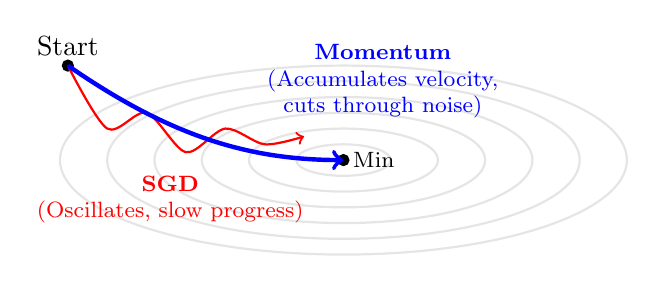
\begin{tikzpicture}[scale=1.0] 
        % --- 1. The Ravine (Elongated Contours) --- 
        \foreach \r in {0.5, 1.0, 1.5, 2.0, 2.5, 3.0} { 
            \draw[gray!20, thick] (4,2) ellipse ({1.2*\r} and {0.4*\r}); 
        } 
        % Minimum 
        \filldraw[black] (4,2) circle (2pt) node[right, font=\footnotesize] {Min}; 
         
        % Start Point 
        \coordinate (start) at (0.5, 3.2); 
        \filldraw[black] (start) circle (2pt) node[above] {Start}; 
 
        % --- 2. SGD Path (Less extreme zigzag, but still inefficient) --- 
        \draw[red, thick, ->] plot[smooth] coordinates { 
            (0.5, 3.2)   % Start 
            (1.0, 2.4)   % slight down 
            (1.5, 2.6)   % slight up 
            (2.0, 2.1)   % down 
            (2.5, 2.4)   % up 
            (3.0, 2.2)   % down
            (3.5, 2.3)   % slight up
        }; 
        \node[red, align=center, font=\footnotesize] at (1.8, 1.5) {\textbf{SGD}\\(Oscillates, slow progress)}; 
 
        % --- 3. Momentum Path (Efficient) --- 
        % Smoothes out the noise and accelerates 
        \draw[blue, ultra thick, ->] (start)  
            .. controls (1.8, 2.3) and (2.8, 2.0) .. (4.0, 2.0); 
        \node[blue, align=center, font=\footnotesize] at (4.5, 3.0) {\textbf{Momentum}\\(Accumulates velocity,\\cuts through noise)}; 
 
    \end{tikzpicture} 
     
    \vspace{0.5em} 
    \begin{tcolorbox}[colback=blue!5, colframe=blue!40, title=The Solution] 
                We add \textbf{Momentum}, which acts like a heavy ball rolling downhill, building velocity and ignoring small bumps. \\It maintains a \textbf{running average} of past gradients ($v_t$), allowing oscillations in opposing directions to cancel out while consistent directions accumulate and accelerate.
 
    \end{tcolorbox} 
\end{frame}

% --- Momentum: Math ---
\begin{frame}{Momentum: Update Rule}
\textbf{Keep a moving average of past gradients:}
\[
v_t = \underbrace{\beta v_{t-1}}_{\text{past gradients}} + \underbrace{(1 - \beta) \nabla_\theta J(\theta)}_{\text{new gradient}}
\]
\[
\theta_{t+1} = \theta_t - \alpha v_t
\]
\begin{itemize}
\item $v_t$ is the \textbf{velocity} (momentum term)
\item $\beta$ is the momentum coefficient (typically 0.9)
\item $\alpha$ is the learning rate
\end{itemize}
\end{frame}

% --- AdaGrad: Intuition ---
\begin{frame}{AdaGrad: Adaptive Learning Rates}
\textbf{Problem:} Same learning rate for all parameters may not be optimal.

\textbf{Idea:} Give each parameter its own adaptive learning rate based on its gradient history.

\vspace{0.5em}
\centering
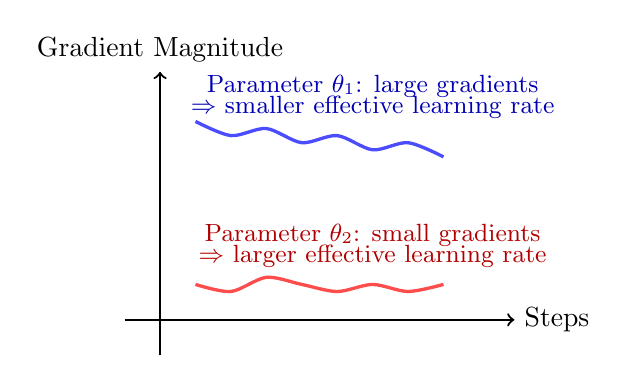
\begin{tikzpicture}[scale=0.9]
    % Two parameters with different gradient histories
    \draw[->, thick] (-0.5,0) -- (5,0) node[right] {Steps};
    \draw[->, thick] (0,-0.5) -- (0,3.5) node[above] {Gradient Magnitude};
    
    % Parameter 1: large, frequent gradients
    \draw[blue!70, very thick, smooth] plot coordinates {
        (0.5, 2.8) (1, 2.6) (1.5, 2.7) (2, 2.5) (2.5, 2.6) (3, 2.4) (3.5, 2.5) (4, 2.3)
    };
    \node[blue!70!black, font=\small] at (3, 3.3) {Parameter $\theta_1$: large gradients};
    \node[blue!70!black, font=\small] at (3, 3.0) {$\Rightarrow$ smaller effective learning rate};
    
    % Parameter 2: small, infrequent gradients
    \draw[red!70, very thick, smooth] plot coordinates {
        (0.5, 0.5) (1, 0.4) (1.5, 0.6) (2, 0.5) (2.5, 0.4) (3, 0.5) (3.5, 0.4) (4, 0.5)
    };
    \node[red!70!black, font=\small] at (3.0, 1.2) {Parameter $\theta_2$: small gradients};
    \node[red!70!black, font=\small] at (3.0, 0.9) {$\Rightarrow$ larger effective learning rate};
\end{tikzpicture}

\vspace{0.7em}
Parameters with large gradients get smaller steps (learning rates).\\
This prevents overshooting.
\end{frame}

% --- AdaGrad: Math ---
\begin{frame}{AdaGrad: Update Rule}
\textbf{Accumulate squared gradients for each parameter:}
\[
G_t = \underbrace{G_{t-1}}_{\text{past squared gradients}} + \underbrace{g_t^2}_{\text{new squared gradient}}
\]
\textbf{Update with parameter-wise learning rate:}
\[
\theta_{t+1} = \theta_t - \underbrace{\frac{\eta}{\sqrt{G_t} + \epsilon}}_{\text{adaptive learning rate}} \, \underbrace{g_t}_{\text{gradient}}
\]
\begin{itemize}
\item $G_t$ accumulates all past squared gradients $\rightarrow$ larger $G_t$ means smaller effective learning rate
\item $\eta$ is the base learning rate
\item $\epsilon$ is a small constant for numerical stability ($\sim 10^{-8}$)
\item Each parameter gets its own effective learning rate
\end{itemize}
\end{frame}

% --- RMSProp: Intuition ---
\begin{frame}{RMSProp: Fixing AdaGrad}
\textbf{Problem with AdaGrad:} Accumulates \textit{all} past gradients $\rightarrow$ Learning rate can shrink too much over time (never forgets past gradients).

\textbf{RMSProp solution:} Use \textbf{exponential moving average} instead (forget old gradients!).

\vspace{0.5em}
\centering
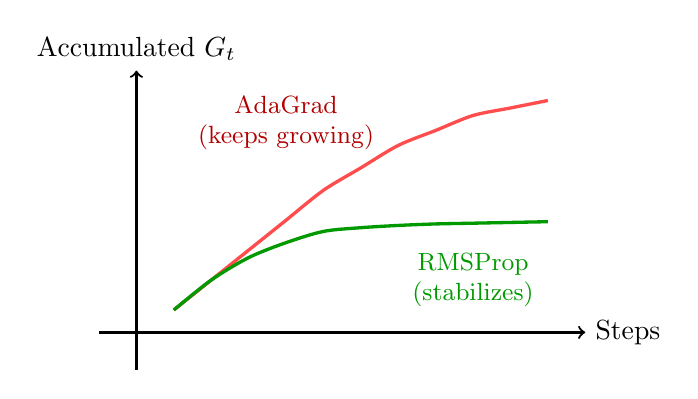
\begin{tikzpicture}[scale=0.95]
    \draw[->, thick] (-0.5,0) -- (6,0) node[right] {Steps};
    \draw[->, thick] (0,-0.5) -- (0,3.5) node[above] {Accumulated $G_t$};
    
    % AdaGrad - keeps growing
    \draw[red!70, very thick, smooth] plot coordinates {
        (0.5, 0.3) (1, 0.7) (1.5, 1.1) (2, 1.5) (2.5, 1.9) (3, 2.2) (3.5, 2.5) (4, 2.7) (4.5, 2.9) (5, 3.0) (5.5, 3.1)
    };
    \node[red!70!black, font=\small, align=center] at (2, 2.8) {AdaGrad\\(keeps growing)};
    
    % RMSProp - stabilizes
    \draw[green!60!black, very thick, smooth] plot coordinates {
        (0.5, 0.3) (1, 0.7) (1.5, 1.0) (2, 1.2) (2.5, 1.35) (3, 1.4) (3.5, 1.43) (4, 1.45) (4.5, 1.46) (5, 1.47) (5.5, 1.48)
    };
    \node[green!60!black, font=\small, align=center] at (4.5, 0.7) {RMSProp\\(stabilizes)};
\end{tikzpicture}

\vspace{0.7em}
\textbf{Effect:} Learning rate adapts but doesn't vanish $\rightarrow$ training continues effectively!
\end{frame}

% --- RMSProp: Math ---
\begin{frame}{RMSProp: Update Rule}
\textbf{Exponential moving average of squared gradients:}
\[
E[g^2]_t = \underbrace{\alpha E[g^2]_{t-1}}_{\text{decayed past gradients}} + \underbrace{(1 - \alpha) g_t^2}_{\text{new squared gradient}}
\]
\textbf{Update rule:}
\[
\theta_{t+1} = \theta_t - \underbrace{\frac{\eta}{\sqrt{E[g^2]_t} + \epsilon}}_{\text{adaptive learning rate}} \, \underbrace{g_t}_{\text{gradient}}
\]
\begin{itemize}
\item $\alpha$ is the decay rate (typically 0.9) (old gradients gradually fade away)
\item Recent gradients have more influence than old ones
\end{itemize}
\end{frame}

% --- Adam: Intuition ---
\begin{frame}{Adam: Best of Both Worlds}
\textbf{Idea:} Combine \textbf{momentum} + \textbf{adaptive learning rates}!
% \vspace{2.5em}
\centering
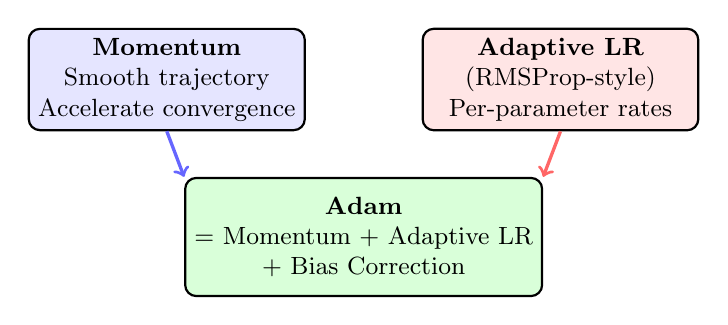
\begin{tikzpicture}[
    box/.style={draw, rounded corners, thick, minimum width=3.5cm, minimum height=1.2cm, align=center, font=\small},
]
    % Momentum box
    \node[box, fill=blue!10] (mom) at (-2.5, 1.5) {\textbf{Momentum}\\Smooth trajectory\\Accelerate convergence};
    
    % Adaptive LR box
    \node[box, fill=red!10] (ada) at (2.5, 1.5) {\textbf{Adaptive LR}\\(RMSProp-style)\\Per-parameter rates};
    
    % Adam box
    \node[box, fill=green!15, minimum width=4.5cm, minimum height=1.5cm] (adam) at (0, -0.5) {\textbf{Adam}\\= Momentum + Adaptive LR\\+ Bias Correction};
    
    % Arrows
    \draw[->, very thick, blue!60] (mom.south) -- (adam.north west);
    \draw[->, very thick, red!60] (ada.south) -- (adam.north east);
\end{tikzpicture}

% \vspace{0.8em}
\textbf{Bias Correction:} At the start of training, moving averages are initialized to zero, causing them to be biased toward zero. Adam corrects this bias to get accurate estimates in early steps.

\vspace{0.5em}
\textbf{Result:} Fast, stable, and works well across many problems (the most popular optimizer in deep learning!)
\end{frame}

% --- Adam: Math ---
\begin{frame}{Adam: Update Rule}
\textbf{Maintain two moving averages:}
\[
m_t = \underbrace{\beta_1 m_{t-1}}_{\text{past momentum}} + \underbrace{(1 - \beta_1) g_t}_{\text{new gradient}} \quad \text{(momentum)}
\]
\[
v_t = \underbrace{\beta_2 v_{t-1}}_{\text{past variance}} + \underbrace{(1 - \beta_2) g_t^2}_{\text{new squared gradient}} \quad \text{(adaptive LR)}
\]

\textbf{Bias correction} (fixes initial zero bias):
\[
\hat m_t = \frac{m_t}{1 - \beta_1^t}, \qquad \hat v_t = \frac{v_t}{1 - \beta_2^t}
\]
{\footnotesize As $t \to \infty$, $\beta^t \to 0$, so correction factor $\to 1$ (no correction needed later)}

\textbf{Update:}
\[
\theta_{t+1} = \theta_t - \underbrace{\frac{\eta}{\sqrt{\hat v_t} + \epsilon}}_{\text{adaptive step size}} \, \underbrace{\hat m_t}_{\text{momentum direction}}
\]
\begin{itemize}
\item Typical: $\beta_1 = 0.9$, $\beta_2 = 0.999$
\end{itemize}
\end{frame}
% --- AdamW: Intuition ---
\begin{frame}{AdamW: Improved Regularization}
\textbf{Problem with Adam:} Weight decay (L2 regularization) interacts poorly with adaptive learning rates.

\textbf{Why?} In Adam, weight decay is added to the gradient before the adaptive scaling. This means parameters with small gradients get disproportionately large weight decay, breaking the intended regularization.

\vspace{0.5em}
\centering
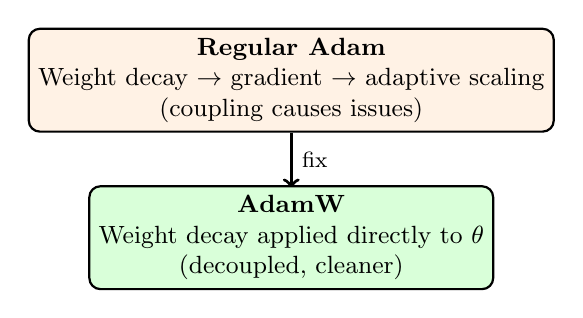
\begin{tikzpicture}[
    box/.style={draw, rounded corners, thick, minimum width=4.2cm, minimum height=1.1cm, align=center, font=\small},
]
    % Regular Adam
    \node[box, fill=orange!10] (adam) at (0, 1.5) {\textbf{Regular Adam}\\Weight decay $\to$ gradient $\to$ adaptive scaling\\(coupling causes issues)};
    
    % Arrow
    \draw[->, very thick] (adam.south) -- ++(0, -0.7) node[midway, right, font=\footnotesize] {fix};
    
    % AdamW
    \node[box, fill=green!15] (adamw) at (0, -0.5) {\textbf{AdamW}\\Weight decay applied directly to $\theta$\\(decoupled, cleaner)};
\end{tikzpicture}

\vspace{0.8em}
\textbf{Result:} Better generalization, especially for large models (current best practice for training modern neural networks!)
\end{frame}

% --- AdamW: Math ---
\begin{frame}{AdamW: Update Rule}
\textbf{Same as Adam, plus decoupled weight decay:}
\[
\theta_{t+1} = \theta_t - \underbrace{\frac{\eta}{\sqrt{\hat v_t} + \epsilon} \, \hat m_t}_{\text{Adam update}} \; - \; \underbrace{\eta \lambda \theta_t}_{\text{weight decay (decoupled)}}
\]

\begin{itemize}
\item First term: standard Adam update (gradient-based optimization)
\item Second term: direct weight decay applied to parameters, independent of gradients
\item $\lambda$ is the weight decay coefficient (typically $0.01$)
\end{itemize}

\textbf{Why better?} Cleaner separation of optimization and regularization.

\end{frame}

% --- Summary Slide (Fixed Spacing) ---
\begin{frame}{Optimizer Summary}
\textbf{Evolution of Optimizers:}
\centering
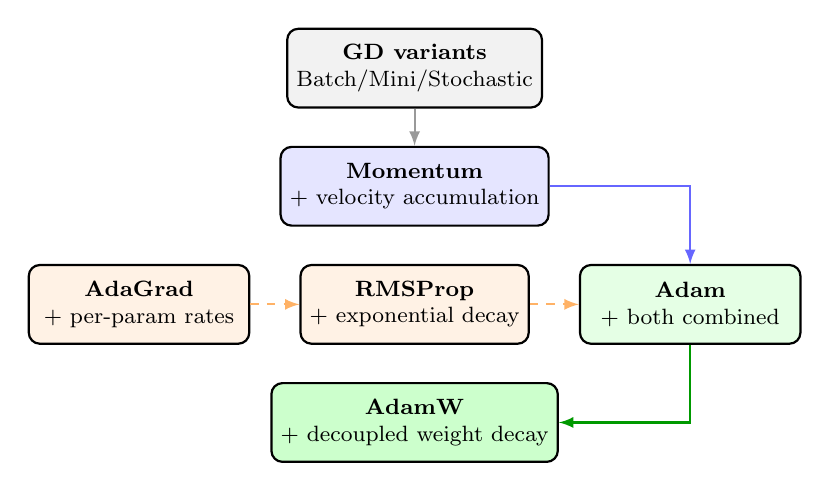
\begin{tikzpicture}[
    box/.style={draw, rounded corners, thick, minimum width=2.8cm, minimum height=1.0cm, align=center, font=\footnotesize},
    >=latex
]
    % 1. Top Nodes (Vertical Backbone)
    \node[box, fill=gray!10] (gd) at (0, 3.5) {\textbf{GD variants}\\Batch/Mini/Stochastic};
    \node[box, fill=blue!10] (mom) at (0, 2.0) {\textbf{Momentum}\\+ velocity accumulation};
    
    % 2. Middle Row (Spread out horizontally to fix overlap)
    % Increased x-distance from 2.5 to 3.5
    \node[box, fill=orange!10] (ada) at (-3.5, 0.5) {\textbf{AdaGrad}\\+ per-param rates};
    \node[box, fill=orange!10] (rms) at (0, 0.5) {\textbf{RMSProp}\\+ exponential decay};
    \node[box, fill=green!10] (adam) at (3.5, 0.5) {\textbf{Adam}\\+ both combined};
    
    % 3. Bottom Node
    \node[box, fill=green!20] (adamw) at (0, -1.0) {\textbf{AdamW}\\+ decoupled weight decay};
    
    % Arrows
    \draw[->, thick, gray!80] (gd) -- (mom);
    
    % Branching arrows
    % \draw[->, thick, blue!60] (mom) -| (ada); % Square path to left
    % \draw[->, thick, blue!60] (mom) -- (rms);
    \draw[->, thick, blue!60] (mom) -| (adam); % Square path to right
    
    % Evolution arrows (Side-to-side)
    \draw[->, thick, orange!60, dashed] (ada) -- (rms);
    \draw[->, thick, orange!60, dashed] (rms) -- (adam);
    
    % Final arrow
    \draw[->, thick, green!60!black] (adam) |- (adamw);

\end{tikzpicture}

\vspace{0.5em}
\textbf{Rule of thumb:} Start with \textbf{AdamW} (it's the most robust default choice!)
\end{frame}


\section{What We Choose When Building a Neural Network}
